\documentclass[12pt]{article}
\usepackage{graphicx}
\graphicspath{{./images/}}
\usepackage[a4paper, total={7in, 10in}]{geometry}
\usepackage{xcolor}
\usepackage{wrapfig}
% remember to remove this stuff, this is for dark mode
% \definecolor{mygrey}{rgb}{0.1,0.1,0.1}
% \pagecolor{mygrey}
% \color{white}

\title{Analyzing the effect of the weight of the mass on the distance travelled by a projectile on a trebuchet}
\author{}
\date{Febuary 14th 2024}

\begin{document}

\maketitle

\pagebreak
\tableofcontents

\pagebreak
% ok this is where the background starts
\section{Background}
Often times in the modern world, we may to forefully propell stones, balls, and even people long distances. Historically this was done through the use of catapults, and trebuchets. For example, if Ricko wanted to throw a fairly large rock at James's house, he would have to calculate the weight needed on the end of the trebuchet to launch the projectile with enough energy to make it to Jame's house, and dmaage it.

Now I too sometimes need to launch objects such as balls distances, maybe not at houses, but nonetheless I still need to launch them. So I turned to using a catapult to launch these objects for me, however I did not know how much weight I need to put on the end of the catapult in order to launch the projectile the desired Distance. Thus I decided to investigate the relationship between the distance traveled by the projectile, and the mass on the end of the trebuchet.

This IA mainly focuses on kinematics, as it is measuring the effect of the mass on the end, compared to the distance travelled. Which at the scale the  experiment is being conducted on, would be under kinematics.

The equations, and relationships in question here would be all of the kinematic equations, the equations used to determine force, work, energy, and momentum. These will be used to determine the energy, as well as the relationship between the weight on the end of the trebuchet, and the distance it is flung.

In order to answer this question, a trebuchet will be built, and it will launch a tennis ball, with various weights on the end. The distance travelled will be compared and analysed to determine a relationship between the mass on the end of the trebuchet and the distance travlled by the ball.


\section{Designs and Mechanisms of the trebuchet}

% rewrite this later, this makes no sense LMFAO

The trebuchet that was built for the purposes of this experiment resembles a large lever, with a load on one end (the projectile), and the counter weight on the other. When it comes to force applied to one side is equal to the force on the otherwise multipled by the mechanical advantage. Mechanical advantage can be determined by dividing the (distance from load to fulcrum), by the (distance from effort to fulcrum). Letting \(L\) be the distance from load to fulcrum, letting \(E\) be the distance from effort to fulcrum, and letting the force being experienced by the projectile be represented by \(F\). The equation ends up as;

The trebuchet that will be built for the purposes of this experiment resembles a large lever, with a load on one end (projectile), and a load on the other end (counter-weight). To determine the force (\(F_{i}\)) which is experienced by the projectile to calculate its acceleration (\(a_{i}\)), and instanous-velocity (\(v_{i}\)) at launch time. The force experiencenced by the side with the counter weight, must be multiplied by the mechanical advantage to determine the force. Then to determine the mechanical advantage, the distance from the fulcrum to the projectile (\(d_{p}\)), must be divided by the distance from the fulcrum to the counter weight (\(d_{cw}\)). This results in the equation for instanous acceleration being. Then the \(F_{i}\) must be divided by the weight (\(m_{tennis ball}\)), finally the velocity can be determined by looking at the distance travelled and determine the time taken, and then using that with acceleration and trig to find the \(v_{x}\), and \(v_{y}\) velocity;

% accelleration equation
\[ a_{t} = \frac{d_{p}}{d_{cw}}\cdot9.81\cdot ( m_{cw} - m_{t} ) \cdot \frac{1}{m_{t}}\] \\
Then to determine the time taken to travel from the ground to released, the suvat equation can be used. Afterwards the velocity can be calculated, and the \(x, y\) velcocities calculated.

Then to determine the velocity of the ball upon being released, multiply the velocity of the ball with the time taken to be released. The time taken to be release can also be calculated using the suvat equations,

% time taken
\(s = ut + \frac{1}{2}at^{2}\) So then since inital velocity is 0, then \(s = \frac{1}{2}at^{2}\), then to determine t the equation can be rearranged as \(\sqrt{\frac{2 \cdot s }{a}} = t\)

% velocity
Then because force is constant, acceleration is constant. So then final velocity can be calculatd by using \(v = u + at\)

Then to determine the \(x, y\) velocity, the sin and cos trigonometric functions can be used. \(\sin{\theta}*v = v_{y}\), \(\cos{\theta}*v = v_{x}\)

Then, assuming air resistance is near neglible, we can assume \(v_{x}\) stays constant, and determine the amount of time it was in the air.

Rearraning all these equations leads to the equation

\(s = \frac{1}{2} \cdot ( \frac {d_{p}}{d_{cw}} )(g) \cdot (m_{cw} - m_{t}) \cdot (\frac {1}{m_{t}}) \cdot [ \frac{d_{p}}{d_{cw}} \cdot (m_{cw} - m_{t}) \cdot \frac{1}{m_{t}}]^{-2} \cdot cos^{2}\theta\)

\paragraph{finding velocity}
\begin{wrapfigure}{r}{0.5\textwidth} %this figure will be at the right
  \centering
  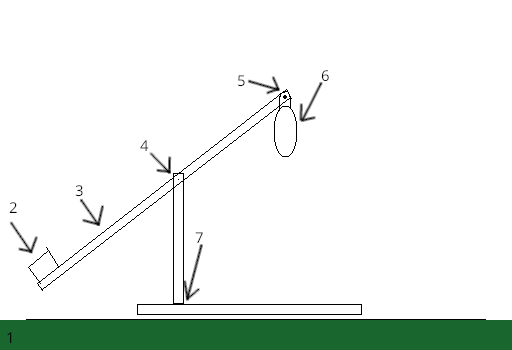
\includegraphics[width=0.5\textwidth]{cataaa}
\end{wrapfigure}


\end{document}
